\documentclass[a4paper, 11pt]{article}
\usepackage{graphicx, float, url, hyperref, lscape, afterpage, amsthm, amsmath}
%\usepackage[margin=1in]{geometry}
\title{Interpolating a Typhoon Trajectory\\ }
\author{CS 236 MP1\\ Joshua Frankie Rayo\\ 2011-19612\\ Scientific Computing Laboratory}
\date{\today}
\newtheorem{definition}{Definition}

\begin{document}
\maketitle

\begin{abstract}
	In this paper, different interpolation techniques are employed to determine the intermediate position of the eye of a typhoon at any time within the time frame. The best interpolant closely resembles the natural path of a typhoon. The trajectory is described as a vector-valued function $f : \mathbf{R} \mapsto \mathbf{R}^2$ that maps a given time to the position of a typhoon. The typhoon track data of Typhoon Haiyan is used in this particular problem.
\end{abstract}

\tableofcontents
\listoffigures
\listoftables

\section{Introduction}
Typhoon Haiyan's activity dates back from November 08 to November 11, 2013 that affected Western Pacific Ocean, Micronesia, Philippines, South China Sea, Northern Vietnam and China. Information about the position of the eye is only available at 6-hour intervals of the specified time frame.

The need for interpolation arises when the position of the eye should be determined on a specific time, obviously not given. We are looking for the best interpolant which can be described as a vector-valued function $f : \mathbf{R} \mapsto \mathbf{R}^2$ that gives the position of the eye given any time within the specified time frame. However, this is only one of the several approaches to solve this problem.

This is useful for typhoon field analysis and in storm surge model simulations as meteorological forcing where $dt$ should be sufficiently small.

\section{Preliminaries}
%\subsection{Typhoon Track Tendencies}
\subsection{Definition of Vector Function}
Consider a particle moving in a plane so that the coordinates $(x, y)$ of its position at any time $t$ are given by the equations
$$ x = \phi(t) \; \mathrm{and} \; y = \lambda(t)$$

A vector exists for any position of the particle, and the endpoints of the position representations of these vectors trace a curve traveled by the particle. This concept leads us to consider a function whose domain is a set of real numbers and whose range is a set of vectors. Such a function is called a \textit{vector-valued function}.

\begin{definition}
	Definition of a Vector-Valued Function.
\end{definition}
Let $\phi$ and $\lambda$ be real-valued functions of a real variable $t$. In the plane, there is a \textbf{vector-valued function} $\mathbf{R}$, defined by
$$\mathbf{R}(t) = \phi(t)\mathbf{\hat{i}} + \lambda(t)\mathbf{\hat{j}}$$
where $t$ is in the domain common to $\phi$ and $\lambda$.

\subsection{Orthogonal Polynomials}
Orthogonal polynomials are yet another useful type of basis functions.

\begin{definition}
	Definition of the inner product
\end{definition}
The inner product $(p, q)$ of two polynomials $p$ and $q$ on an interval $[a,b]$ is defined by
$$ (p, q) = \int_{a}^{b} p(t)q(t)w(t) dt$$
where $w(t)$ is a nonnegative \textit{weight function}, and $p$ and $q$ are said to be \textit{orthogonal} if $(p, q)=0$.

Furthermore, a set of polynomials $\lbrace{p_i}\rbrace$ are \textit{orthonormal} if
$$(p_i, p_j) = 
\begin{cases}
	1, i = j \\
	0, i \neq j.
\end{cases}
$$

Given a set of polynomials, the Gram-Schmidt orthogonalization process can be used to generate an orthonormal set spanning the same space.

\subsection{Hermite Orthogonal Polynomials}

Hermite polynomials \cite{bib:hermite} can be generated using the following definition:
$$H_n(x) = e^{-x^2/2}\left(x-\frac{d}{dx}\right)^{n}e^{x^2/2}$$
The first few Hermite Polynomials $\lbrace{H_n}\rbrace$ are:
\begin{align*}
& H_0(x)=1\\
& H_1(x)=2x\\
& H_2(x)=4x^2-2\\
& H_3(x)=8x^3-12x\\
& H_4(x)=16x^4-48x^2+12\\
& H_5(x)=32x^5-160x^3+120x\\
& H_6(x)=64x^6-480x^4+720x^2-120\\
& H_7(x)=128x^7-1344x^5+3360x^3-1680x\\
& H_8(x)=256x^8-3584x^6+13440x^4-13440x^2+1680\\
& H_9(x)=512x^9-9216x^7+48384x^5-80640x^3+30240x\\
& H_{10}(x)=1024x^{10}-23040x^8+161280x^6-403200x^4+302400x^2-30240
\end{align*}

They are orthogonal in the range $(-\infty,\infty)$ with respect to the weighting function $e^{-x^2}$
$$\int_{-\infty}^{\infty}H_i(x)H_j(x)e^{-x^2}dx=\delta_{ij}2^{j}j!\sqrt{\pi}, \ i\neq j$$
where $\delta_{ij}$ is the Delta function \cite{bib:delta} defined by
$$\delta_{ij}=\delta(i,j)=
\begin{cases}
0, i \neq j \\
1, i = j
\end{cases}
$$
They satisfy the symmetry condition
$$H_n(-x)=(-1)^{n}H_n(x)$$
They also obey the recurrence relations
$$H_{n+1}(x) = 2xH_n(x)-2nH_{n-1}(x)$$
$$H'_n(x)=2nH_{n-1}(x)$$

\section{Case Study: Typhoon Haiyan}
\subsection{Track Data}
Usually, the track data has the format RSMC Best Track Data, with specifications from \cite{bib:track}. Real data is obtained from the Joint Typhoon Warning Center \cite{bib:trackdata} which monitors typhoons using their satellites. This paper only concerns position and time, so irrelevant data are removed:

\begin{table}[H]
	\centering
	\begin{tabular}[H]{c | c c}
		\textit{Time (t)} & &\\
		\textit{(MMDDHH)} & \textit{Lat} $(\phi)$ & \textit{Lon} $(\lambda)$ \\
		\hline
		110400 & 6.1N & 151.5E \\
		110406 & 6.1N & 150.1E \\
		110412 & 6.3N & 148.7E \\
		110418 & 6.4N & 147.2E \\
		110500 & 6.4N & 145.7E \\
		110506 & 6.5N & 144.2E \\
		110512 & 6.9N & 142.9E \\
		110518 & 7.1N & 141.3E \\
		110600 & 7.3N & 139.7E \\
		110606 & 7.6N & 138.0E \\
		110612 & 7.9N & 136.1E \\
		110618 & 8.2N & 134.3E \\
		110700 & 8.7N & 132.7E \\
		110706 & 9.4N & 131.0E \\
		110712 & 10.2N & 129.0E \\
		110718 & 10.6N & 126.9E \\
		110800 & 11.0N & 124.7E \\
		110806 & 11.4N & 122.5E \\
		110812 & 11.8N & 120.4E \\
		110818 & 12.4N & 117.9E \\
		110900 & 12.6N & 116.2E \\
		110906 & 13.4N & 114.6E \\
		110912 & 14.5N & 113.1E \\
		110918 & 15.5N & 111.5E \\
		111000 & 16.5N & 110.1E \\
		111006 & 17.9N & 109.2E \\
		111012 & 19.3N & 108.0E \\
		111018 & 20.5N & 107.4E \\
		111100 & 21.8N & 107.3E \\
		111106 & 23.2N & 107.9E \\
	\end{tabular}
	\caption{Position of typhoon Haiyan through time}
	\label{tbl:pos}
\end{table}

Graphical representation can be obtained from \cite{bib:trackgraph}, and is given below.

\begin{center}
	\begin{figure}[H]
		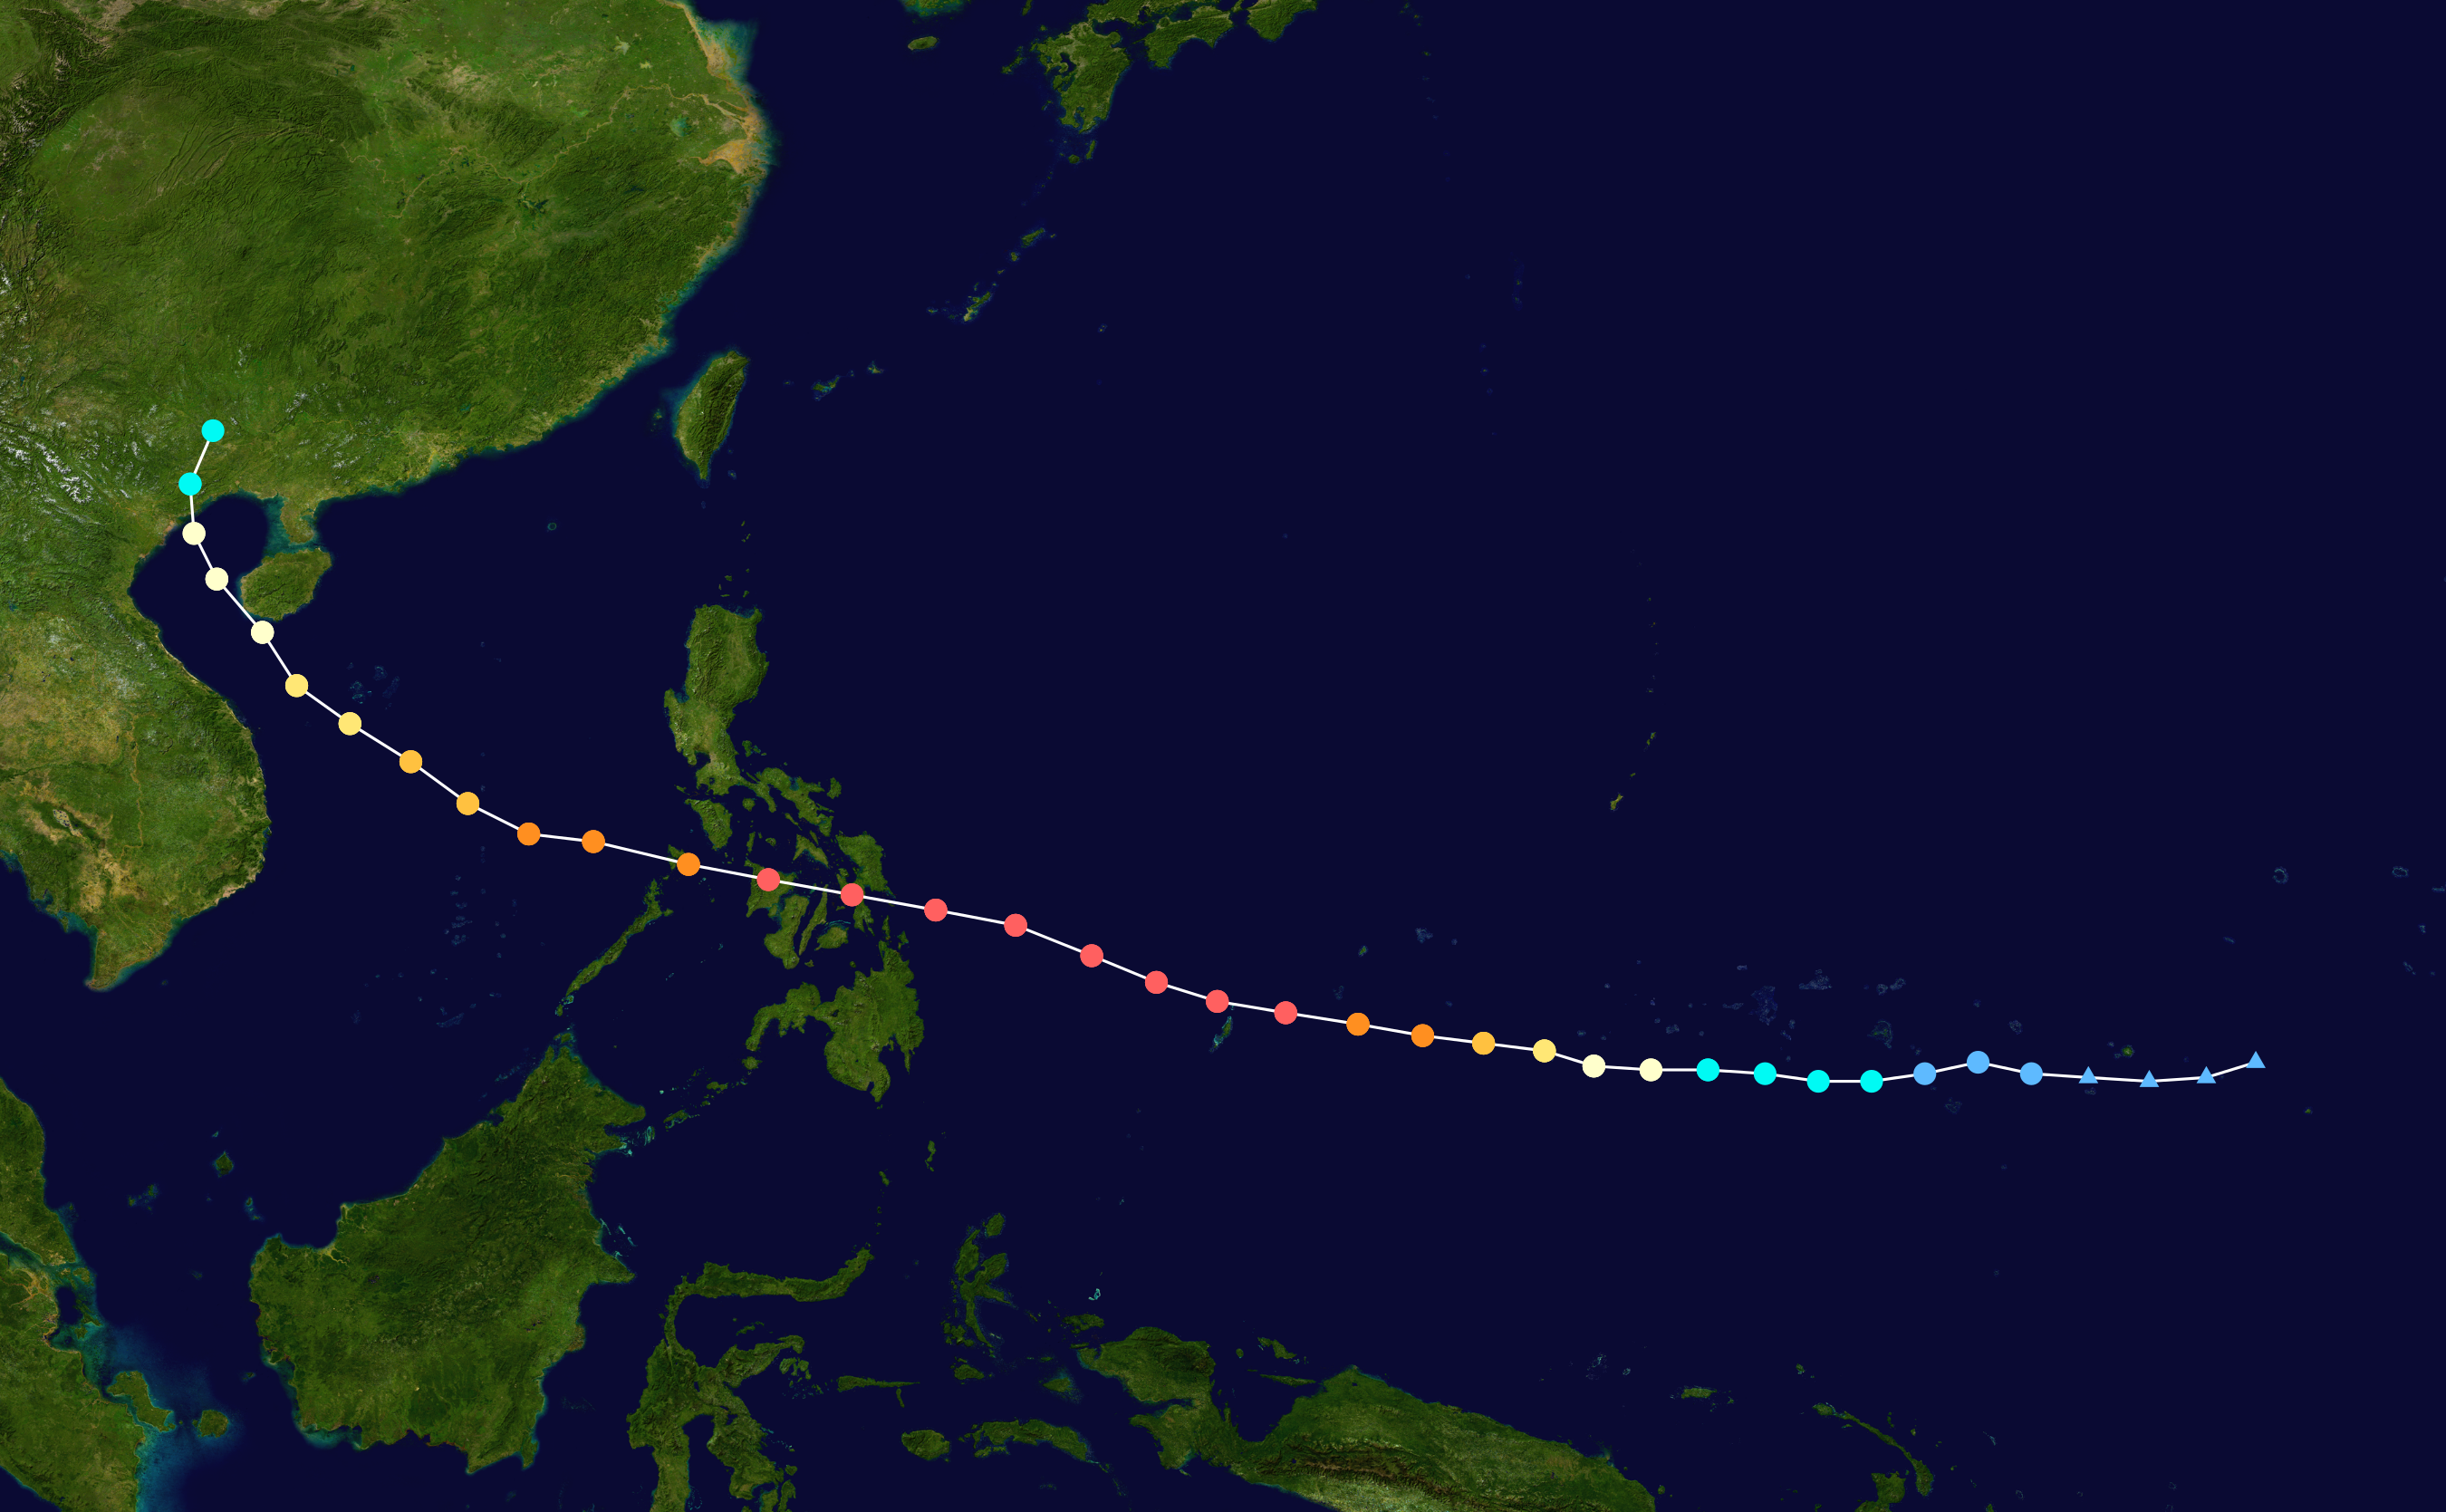
\includegraphics[width=\textwidth]{track}
		\caption{Track of typhoon Haiyan}
	\end{figure}
\end{center}

\section{Methodology}
\subsection{Assumptions}
We are concerned with the movement of typhoon in a spherical surface. Therefore, we utilize the spherical coordinate system $(\rho, \phi, \lambda)$. However, we assume $\rho$ is constant; so the coordinate system will be reduced to $(\phi, \lambda)$.

Note that forecasting or extrapolation are not relevant to the study. Time $t$ will be the time relative to the starting time of the typhoon. North and East will be of positive (+) signs and West and South will be of negative signs (-). Typhoon's position will depend on time only. We will interpolate the position every 1 hour. Modifying table \ref{tbl:pos} above, we have now the following table of values:
\begin{table}[H]
	\centering
	\begin{tabular}{c | c c}
		\textit{Time (t)} & \textit{Lat} $(\phi)$ & \textit{Lon} $(\lambda)$ \\
		\hline
		0 & 6.1 & 151.5 \\
		6 & 6.1 & 150.1 \\
		12 & 6.3 & 148.7 \\
		18 & 6.4 & 147.2 \\
		24 & 6.4 & 145.7 \\
		30 & 6.5 & 144.2 \\
		36 & 6.9 & 142.9 \\
		42 & 7.1 & 141.3 \\
		48 & 7.3 & 139.7 \\
		54 & 7.6 & 138.0 \\
		60 & 7.9 & 136.1 \\
		66 & 8.2 & 134.3 \\
		72 & 8.7 & 132.7 \\
		78 & 9.4 & 131.0 \\
		84 & 10.2 & 129.0 \\
		90 & 10.6 & 126.9 \\
		96 & 11.0 & 124.7 \\
		102 & 11.4 & 122.5 \\
		108 & 11.8 & 120.4 \\
		114 & 12.4 & 117.9 \\
		120 & 12.6 & 116.2 \\
		126 & 13.4 & 114.6 \\
		132 & 14.5 & 113.1 \\
		138 & 15.5 & 111.5 \\
		144 & 16.5 & 110.1 \\
		150 & 17.9 & 109.2 \\
		156 & 19.3 & 108.0 \\
		162 & 20.5 & 107.4 \\
		168 & 21.8 & 107.3 \\
		174 & 23.2 & 107.9 \\
	\end{tabular}
	\caption{Modified table of values from table \ref{tbl:pos}}
	\label{tbl:table}
\end{table}

Given these assumptions, we are now ready to look for the vector-valued function
$$P(t) = (\phi(t), \lambda(t))$$
subject to the following constraints
\begin{eqnarray}
t \in [0, 174] \\
\phi \in [-90, 90] \\
\lambda \in \left(-180, 180\right]
\end{eqnarray}

The key step is to interpolate $\phi$ and $\lambda$ given $t$ to obtain the vector-valued function. This is done with different techniques for interpolation:
\subsection{Machine Specifications}
Succeeding computations are done in MATLAB R2015a 64-bit using 64-bit Windows 7 operating system with Intel\textregistered \hfil Core\texttrademark \hfil i3-2310M CPU with 4 logical processors and 8.00GB of RAM.



\subsection{Polynomial Interpolation}

\subsubsection{Lagrange Polynomial Interpolation}
The code \texttt{lagrangeinter.m} shows the three plots that describe the trajectory of the typhoon:
\begin{figure}[H]
	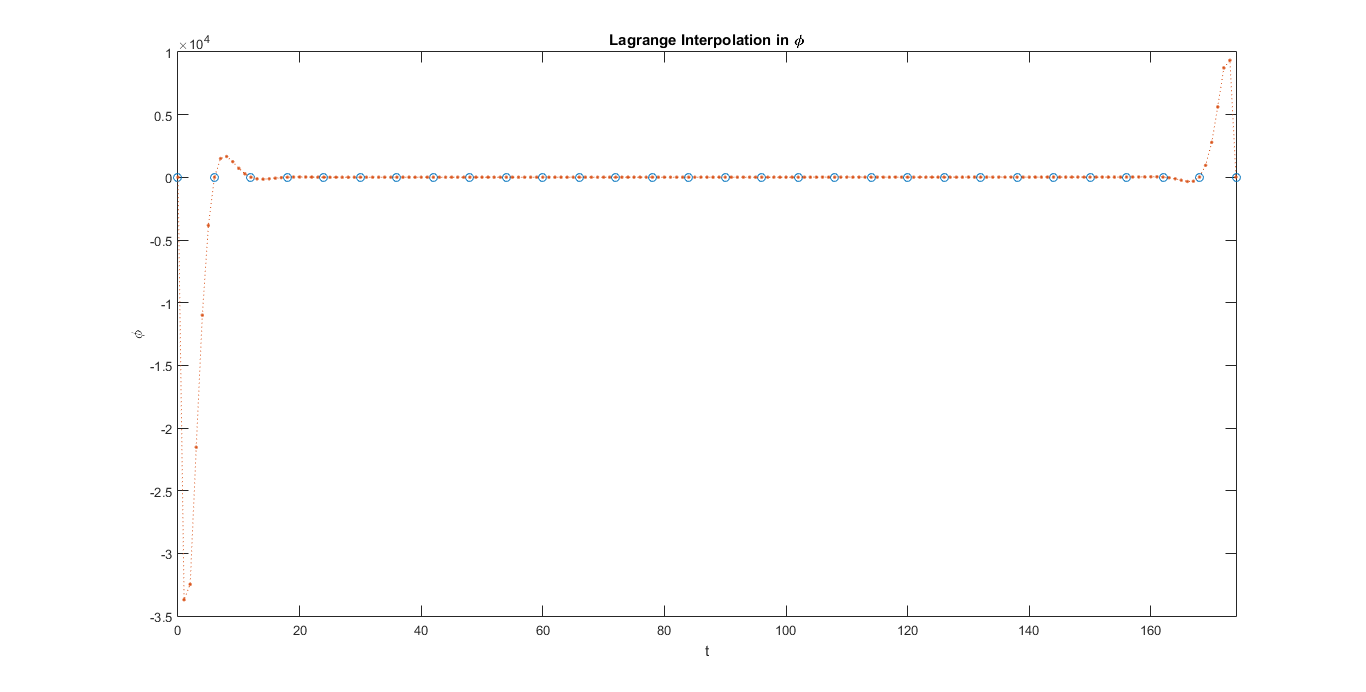
\includegraphics[width=\textwidth]{lagrange/lagrangephi}
	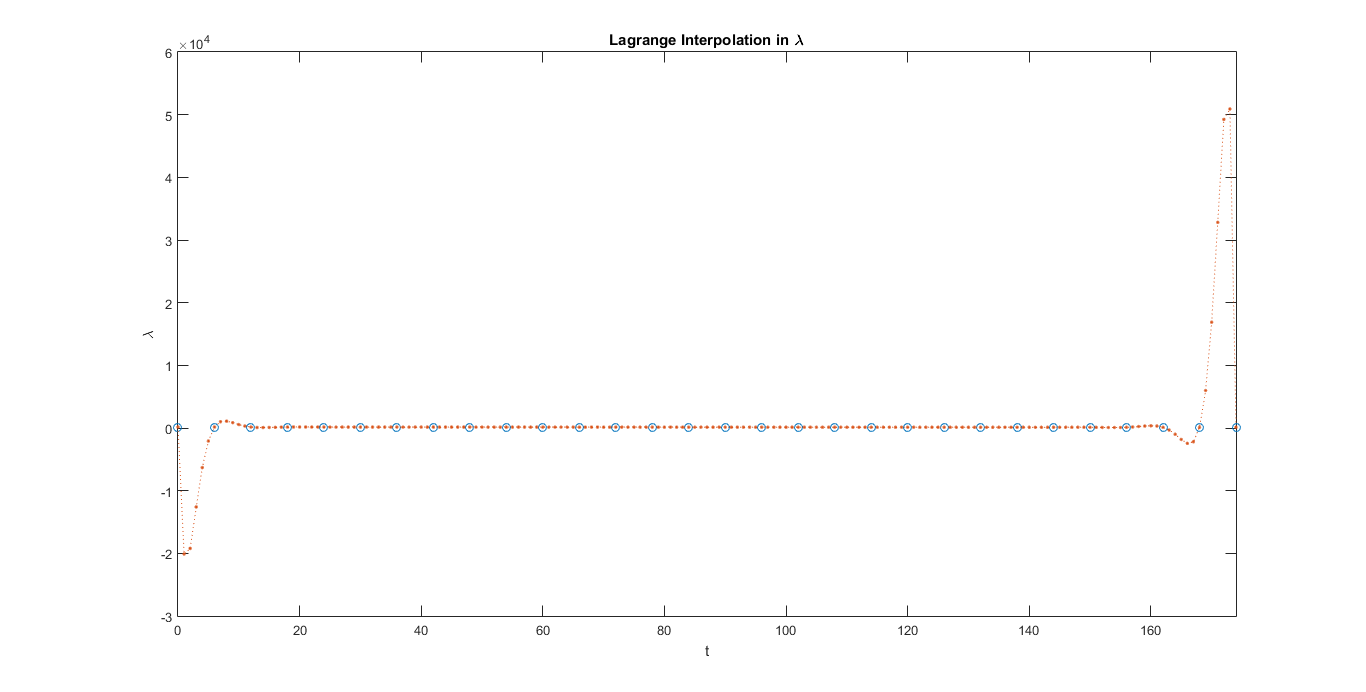
\includegraphics[width=\textwidth]{lagrange/lagrangelambda}
	\caption{Lagrange interpolation in longitude $(\phi)$ and latitude $(\lambda)$}
\end{figure}

The interpolation does not work properly in the interval $t \in [0, 18) \cup (156, 172]$. Because we are using polynomial interpolation, the error goes large and the curve wiggles near the endpoints. Extreme values are in magnitude of $10^4$. The more points we need to interpolate using Lagrange basis, the bigger the error we will get near the endpoints.

\begin{figure}[H]
	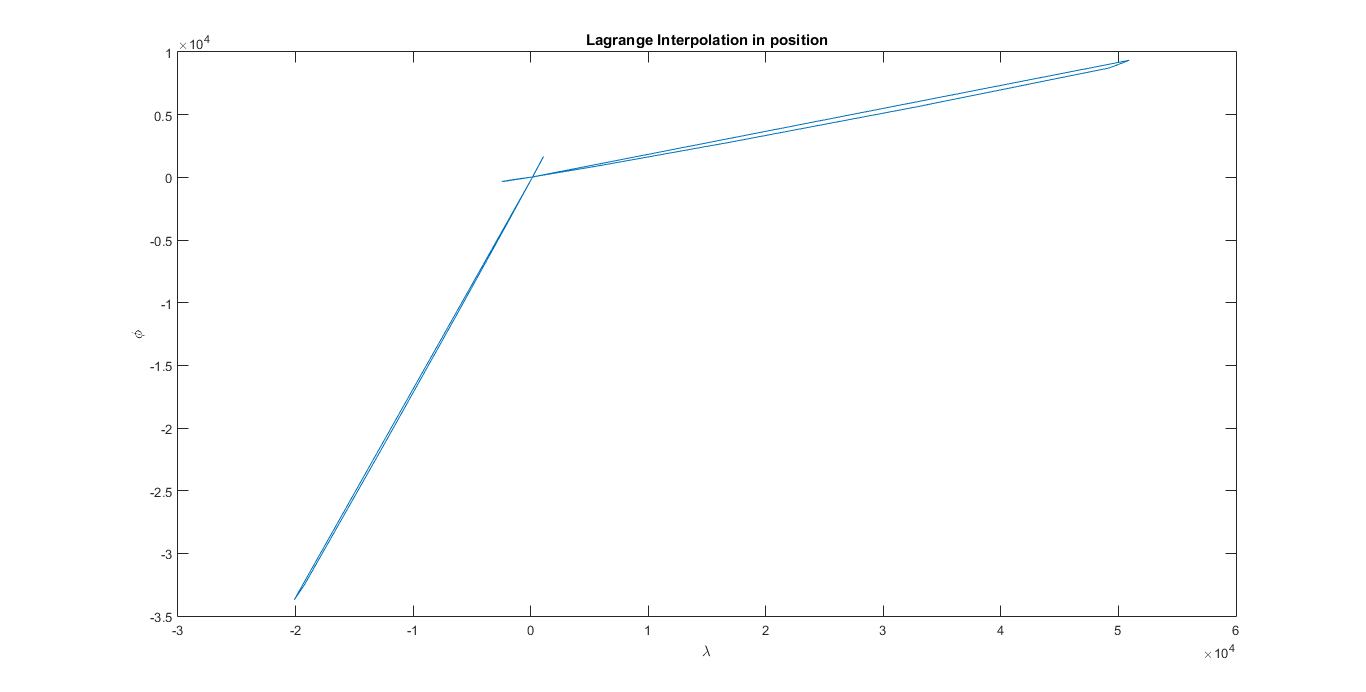
\includegraphics[width=\textwidth]{lagrange/lagrange}
	\caption{Lagrange interpolation in position $(\phi, \lambda)$}
\end{figure}

The trajectory of typhoon will look like this as expected since we have large values of $\phi$ and $\lambda$ when $t$ starts or ends.

Now, we observe the trajectory of the typhoon when $t \in [18, 154]$:
\begin{figure}[H]
	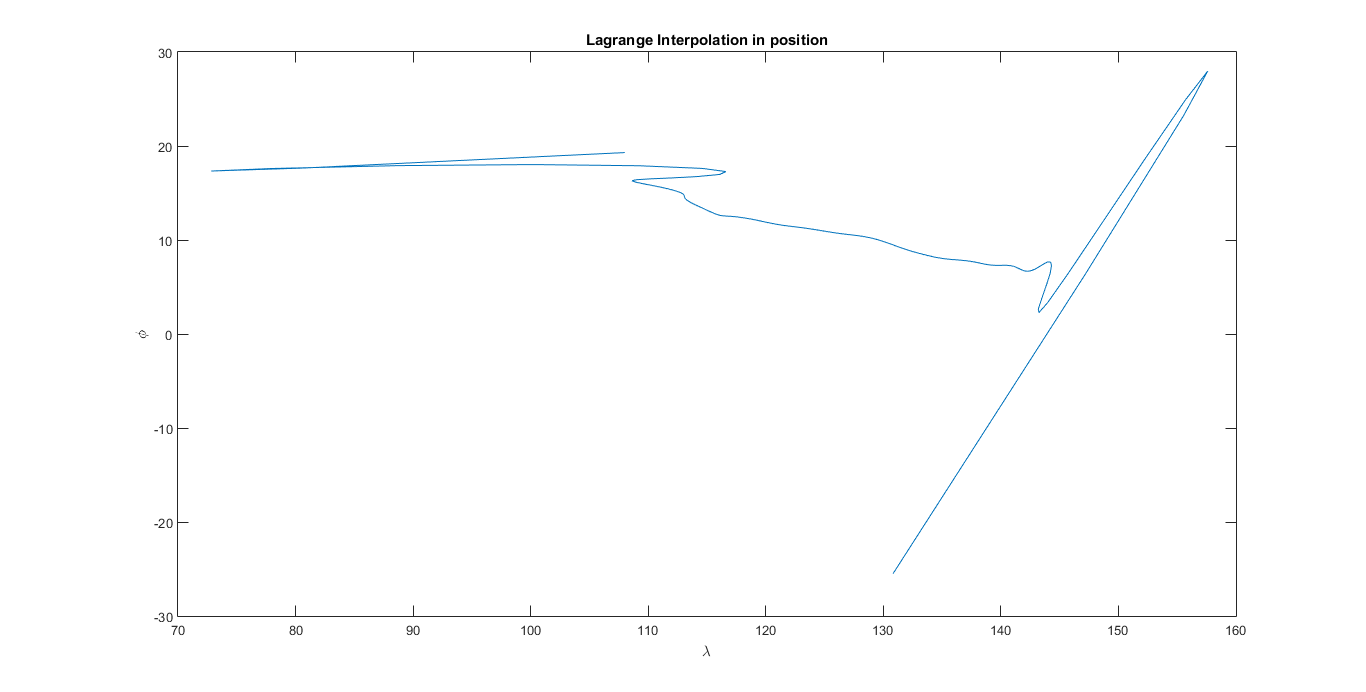
\includegraphics[width=\textwidth]{lagrange/lagrange2}
	\caption{Lagrange interpolation in position $(\phi, \lambda)$ (zoomed in)}
\end{figure}
The trajectory is still inconsistent, suggesting that the polynomial interpolation in general is not a good solution to this problem.

\subsubsection{Hermite Polynomial Interpolation}
In this method, Hermite orthogonal polynomials $\lbrace{H_i}\rbrace$ will be used as basis functions for interpolation. Basically we are looking for the linear combination of basis functions to interpolate the data points.

Suppose we have data points $(t_i, y_i), i=1, 2, \ldots n$ to be interpolated, we need to get $x_i$'s such that:
$$\sum_{i=0}^{i=n}\ x_iH_i(t_i) = y_i$$
In matrix form, we have:
$$
\begin{bmatrix}
1 & H_1(t_1) & \cdots & H_n(t_1) \\
1 & H_1(t_2) & \cdots & H_n(t_2) \\
\vdots  & \vdots  & \ddots & \vdots  \\
1 & H_1(t_n) & \cdots & H_n(t_n) \\
\end{bmatrix}
\begin{bmatrix}
x_1 \\
x_2 \\
\vdots \\
x_n
\end{bmatrix}
=
\begin{bmatrix}
y_1 \\
y_2 \\
\vdots \\
y_n
\end{bmatrix}
$$
The matrix equation above can be represented as $\mathbf{Ax=y}$, and we know that $\mathbf{x=A^{-1}y}$ given that $\mathbf{A}$ is not singular. With this regard, we need to investigate the condition number of $\mathbf{A}$.

In our specific case, $cond(\mathbf{A}) = O(10^{47})$ since there are 26 points to be interpolated. Furthermore, the computation time is considerably slow. It takes about 4 minutes to generate the Hermite orthogonal functions, getting $A$, solving $x$, evaluating $t$ at 1-hour intervals and plotting the graphs.

\begin{figure}[H]
	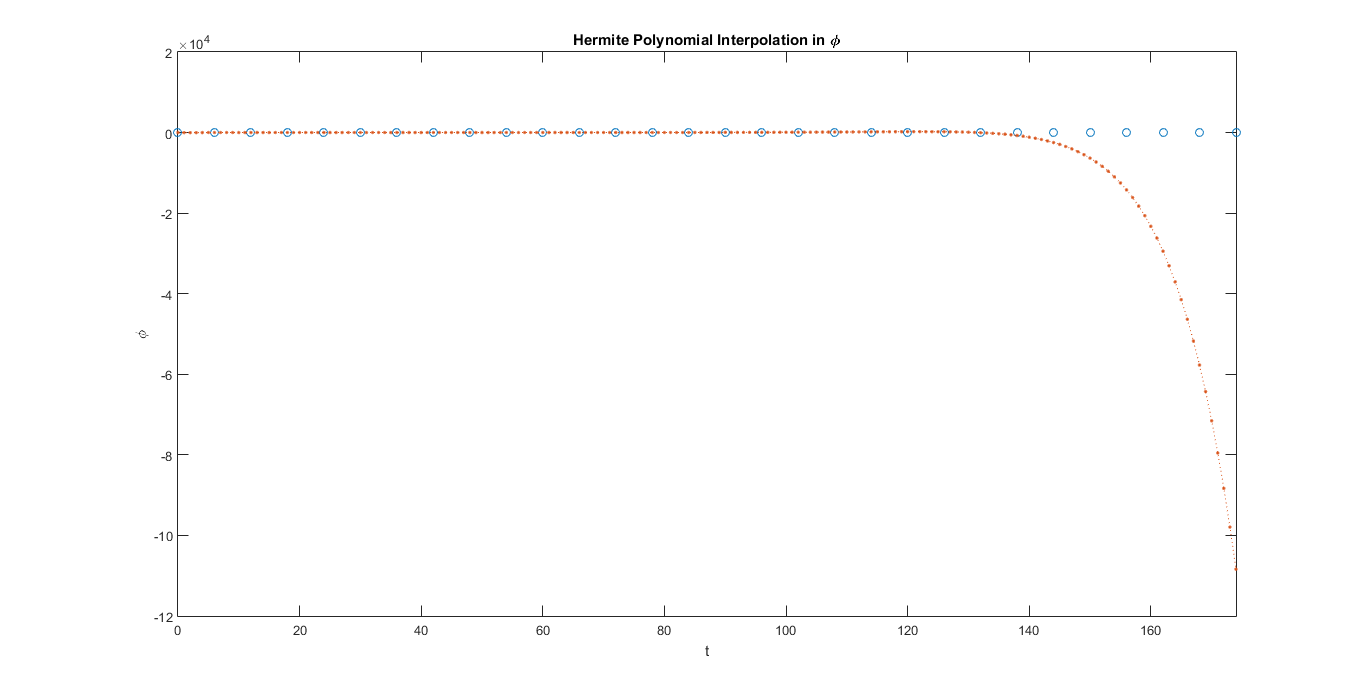
\includegraphics[width=\hsize]{ortho/orthophi}
	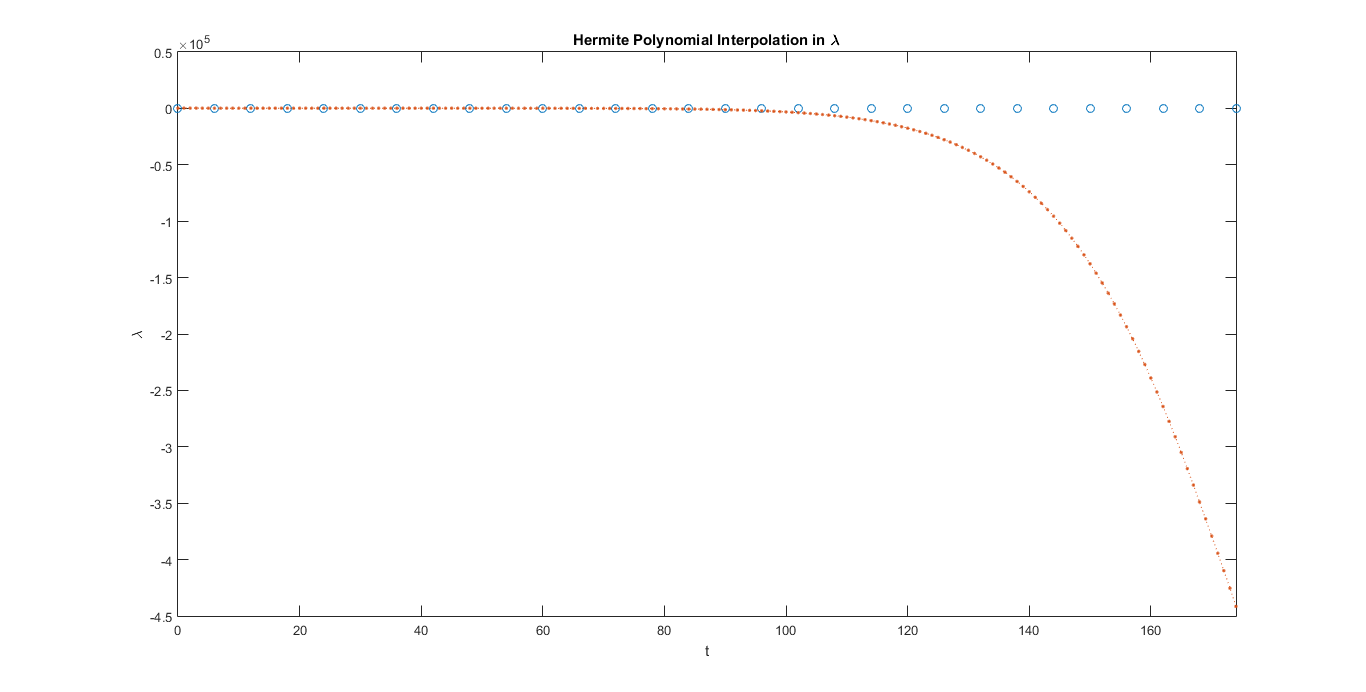
\includegraphics[width=\hsize]{ortho/ortholambda}
	\caption{Hermite orthogonal polynomial interpolation in longitude $(\phi)$ and latitude $(\lambda)$}
\end{figure}

\begin{figure}[H]
	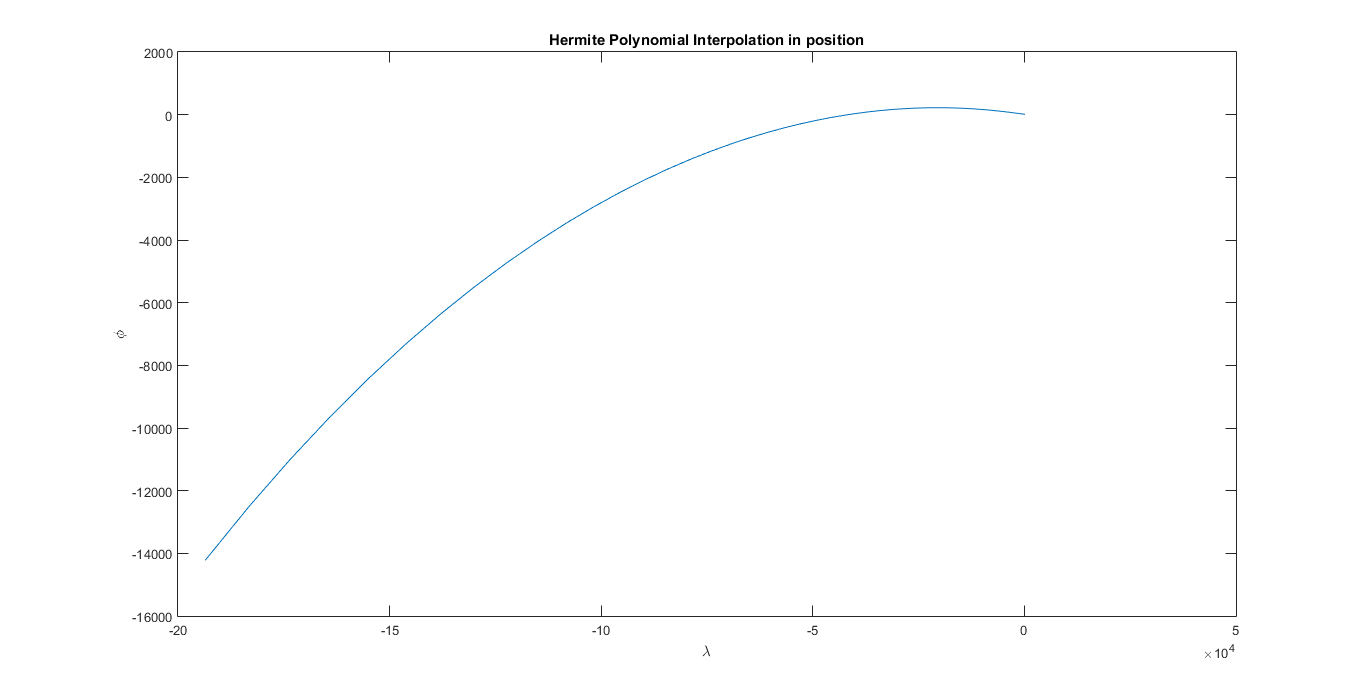
\includegraphics[width=\hsize]{ortho/ortho}
	\caption{Hermite orthogonal polynomial interpolation in position $(\phi, \lambda)$}
\end{figure}

As you can see, interpolation on $\phi$ and $\lambda$ only worked on the first few points then error propagates quickly at the end, compared to Lagrange polynomials where the error propagates at the endpoints.


\subsection{Piecewise Polynomial Interpolation}
\subsubsection{Linear Interpolation}
Simply connect the dots with lines. The code \texttt{linearinter.m} shows the three plots that describe the trajectory of the typhoon:

\begin{landscape}
\begin{figure}[H]
	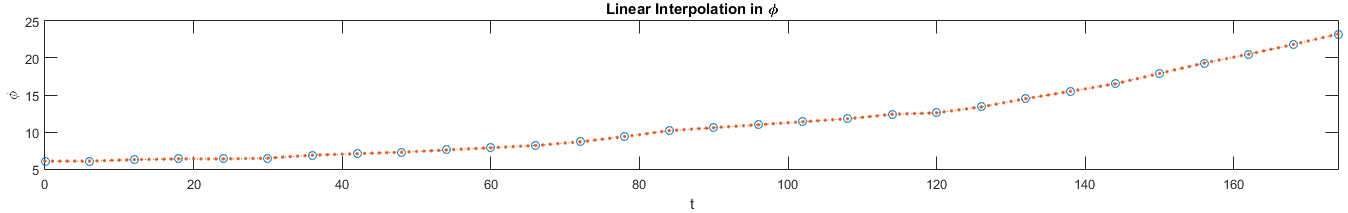
\includegraphics[width=\hsize]{linear/linearphi}
	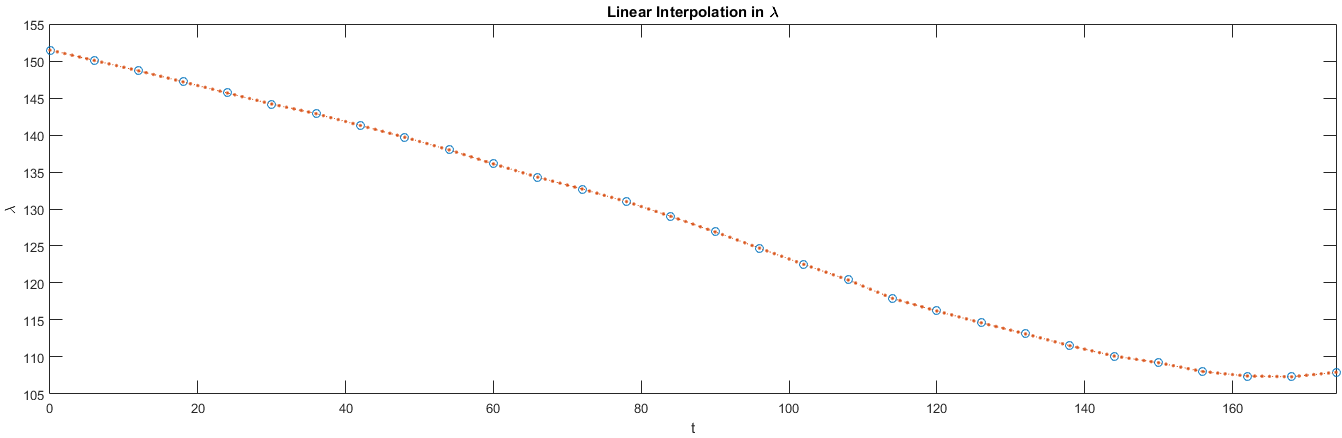
\includegraphics[width=\hsize]{linear/linearlambda}
	\caption{Linear interpolation in longitude $(\phi)$ and latitude $(\lambda)$}
\end{figure}

\begin{figure}[H]
	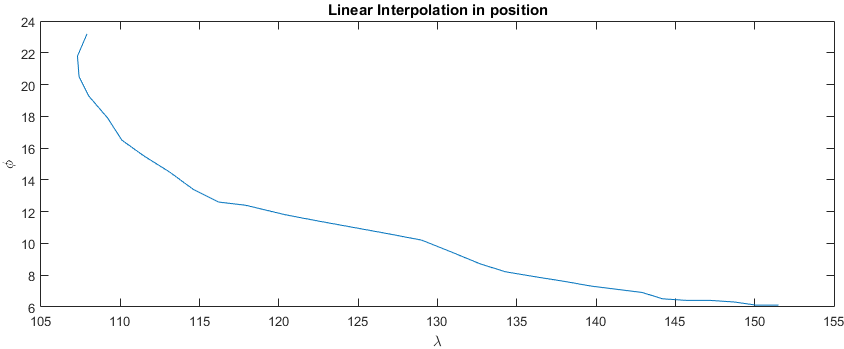
\includegraphics[width=\hsize]{linear/linear}
	\caption{Linear interpolation in position $(\phi, \lambda)$}
\end{figure}

As you can see, $\phi$ and $\lambda$ are piecewise linear, so the interpolant is also piecewise linear. Also note that the interpolated trajectory is now closer to the natural trajectory of the typhoon.
\end{landscape}

\subsubsection{Cubic Spline Interpolation}
Periodic condition is enforced, where the first and second derivatives of the endpoints are equal. The code \texttt{cubicinter.m} shows the three plots that describe the trajectory of the typhoon:
\begin{landscape}
	\begin{figure}[H]
		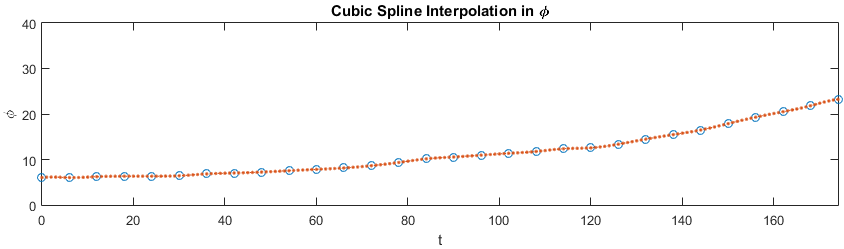
\includegraphics[width=\hsize]{cubic/cubicphi}
		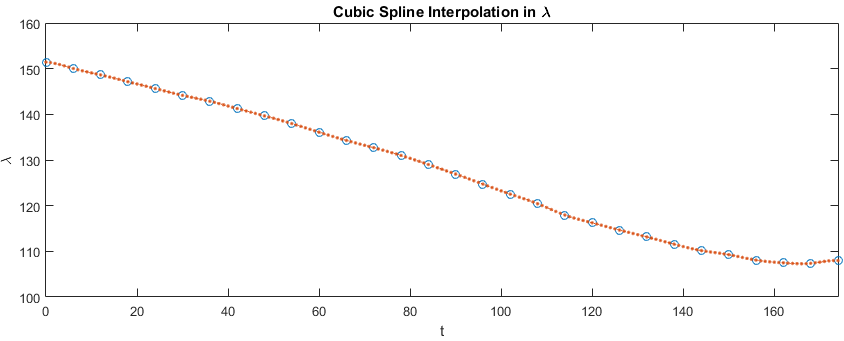
\includegraphics[width=\hsize]{cubic/cubiclambda}
		\caption{Cubic Spline interpolation in longitude $(\phi)$ and latitude $(\lambda)$}
	\end{figure}
	\begin{figure}[H]
		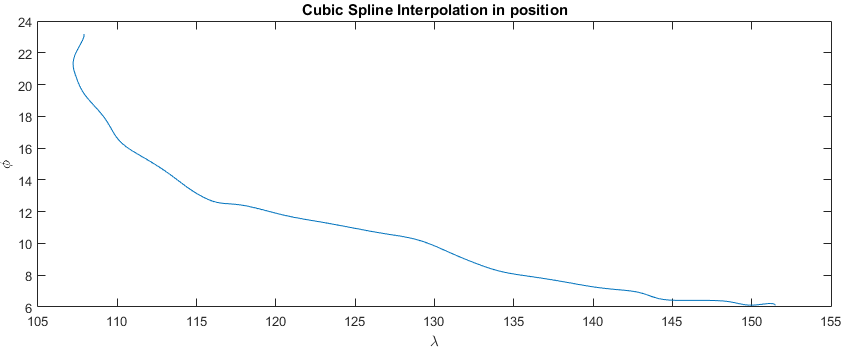
\includegraphics[width=\hsize]{cubic/cubic}
		\caption{Cubic Spline interpolation in position $(\phi, \lambda)$}
	\end{figure}
	As you can see here, the trajectory is quite curvy.
\end{landscape}

\subsubsection{Monotonic Hermite Interpolation}
The monotonic Hermite interpolant has the following characteristics:
\begin{itemize}
	\item On each subinterval $x_i \leq x \leq x_{i+1}$, $P(x)$ is the cubic Hermite interpolant to the given values and certain slopes at the two endpoints
	\item $P(x)$ interpolates y, i.e., $P(x_i)=y_i$, and the first derivative $\frac{dP}{dx}$ is continuous. The second derivative $\frac{d^2P}{dx^2}$ is probably not continuous; there may be jumps at $x_i$.
	\item The slopes at $x_i$ are chosen in such a way that $P(x)$ preserves the shape of the data and is monotonous. On intervals where the data are monotonic, so is $P(x)$; at points where the data has a local extremum, so does $P(x)$.
\end{itemize}
The code \texttt{hermiteinter.m} shows the three plots that describe the position of the typhoon:
\begin{landscape}
	\begin{figure}[H]
		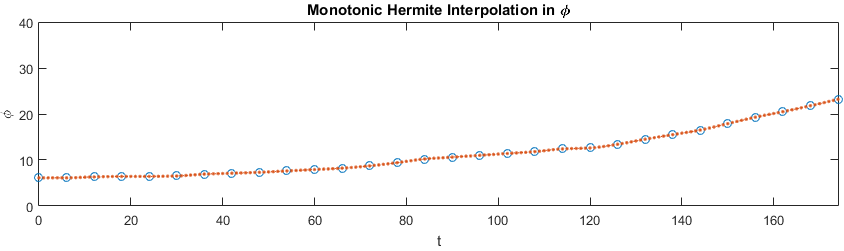
\includegraphics[width=\hsize]{hermite/hermitephi}
		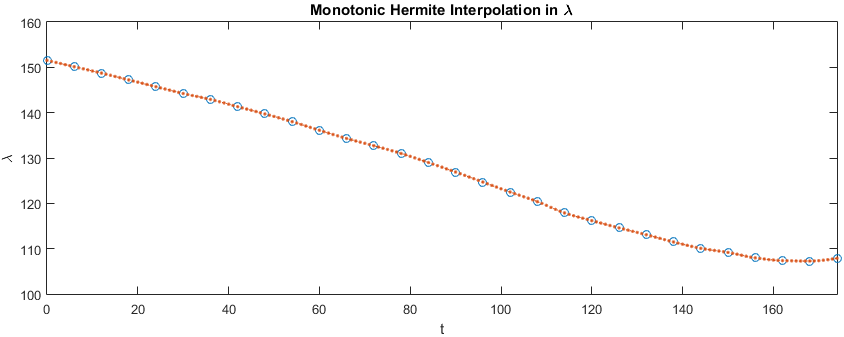
\includegraphics[width=\hsize]{hermite/hermitelambda}
		\caption{Monotonic Hermite interpolation in longitude $(\phi)$ and latitude $(\lambda)$}
	\end{figure}
	\begin{figure}[H]
		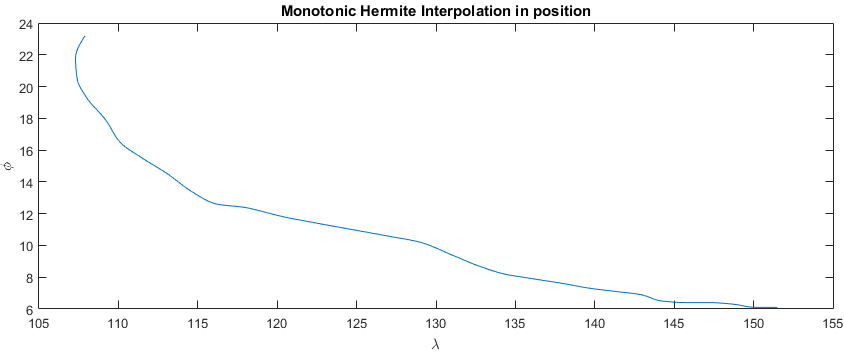
\includegraphics[width=\hsize]{hermite/hermite}
		\caption{Monotonic Hermite interpolation in position $(\phi, \lambda)$}
	\end{figure}
	As you can see here, the trajectory also has curves, but less curvy than the cubic spline interpolant.
\end{landscape}

\section{Results}
It seems that the Monotonic Hermite interpolation performed the best among the interpolation methods described above. The best interpolant $P(t)$ can be represented as piecewise monotonic hermite cubic functions.

\section{Bibliography}
\begin{thebibliography}{9}
	\bibitem{bib:gda}
	Global Disaster Alert and Coordination System, \emph{Typhoon Haiyan}. \url{http://www.gdacs.org/report.aspx?name=HAIYAN}
	
	\bibitem{bib:track}
	Joint Typhoon Warning Center, \emph{Western North Pacific Best Track Data Format}. \url{http://www.usno.navy.mil/NOOC/nmfc-ph/RSS/jtwc/best_tracks/wpindex.php}
	
	\bibitem{bib:trackdata}
	Joint Typhoon Warning Center, \emph{Haiyan Best Track Data}. \url{http://www.usno.navy.mil/NOOC/nmfc-ph/RSS/jtwc/best_tracks/2013/2013s-bwp/bwp312013.dat}
	
	\bibitem{bib:trackgraph}
	Japan Meteorological Agency, \emph{RSMC Best Track Data (Graphics) in 2013}. \url{http://www.jma.go.jp/jma/jma-eng/jma-center/rsmc-hp-pub-eg/bstve_2013_m.html}
	
	\bibitem{bib:hermite}
	Wolfram MathWorld, \emph{Hermite Polynomials}.
	\url{http://mathworld.wolfram.com/HermitePolynomial.html}
	
	\bibitem{bib:delta}
	Wolfram MathWorld, \emph{Kronecker Delta Function}.
	\url{http://mathworld.wolfram.com/KroneckerDelta.html}
	
	\bibitem{bib:tc7}
	Louis Leithold, \emph{The Calculus 7}. Pearson Education Asia Pte. Ltd. 2002
	
	\bibitem{bib:sci}
	Michael Health, \emph{Scientific Computing - An Introductory Survey}. Mc-Graw Hill. 2002
\end{thebibliography}

\end{document}